
 \chapter{\IfLanguageName{dutch}{resultaten}{resultaten}}
\label{ch:Resultaten}
In dit hoofdstuk zullen de resultaten van de testen en de enquête verwerkt worden om zo tot een antwoord te komen op dit onderzoek. Hierbij zijn de resultaten van de Cisco Identity Services Engine omgeving opgedeeld in 'Port-based en Policy-based network access control' en 'Tread-Centric en Policy-based network access control'. Vervolgens zijn de enquête resultaten verwerkt met een aantal diagrammen. Deze resultaten zijn ingedeelt per vraag. 

\section{Cisco Identity Services Engine omgeving}
Zoals men ziet wordt Policy-based network access control steeds gecombineerd met Port-based en Thead-Centric network access control. Dit heeft als rede dat voor zowel Port-based, als voor Thread-Centric network access control, policy rules zijn toegepast.


\subsection{Port-based en Policy-based network access control}
Wanneer 'Port-based en Policy-based network access control' niet zijn toegepast. Dan ziet men dat gebruikers zich kunnen aansluiten op het netwerk zonder enige beveiliging. Natuurlijk moeten de poorten ingesteld worden met het correcte vlan id om trafiek toe te laten. Maar het is enerzijds duidelijk dat het aansluiten op het netwerk via de poorten veel eenvoudiger is. 
\newline
\newline
Als men de resultaten van 'Port-based en Policy-based network access control' er bij halen. Dan ziet men een duidelijk verschil in beveiliging  met of zonder de use cases. Wanneer een gebruiker zich wenst aan te melden op het netwerk via een van de poorten op de fysieke Cisco switch. Dan wordt geen trafiek toegelaten op het netwerk. Dit resulteert in het ontvangen van ip adres van de vorm 169.254.x.x, dat geen enkel compartiment van het netwerk kan bereiken.
 
\begin{figure}[H]
	\centering
	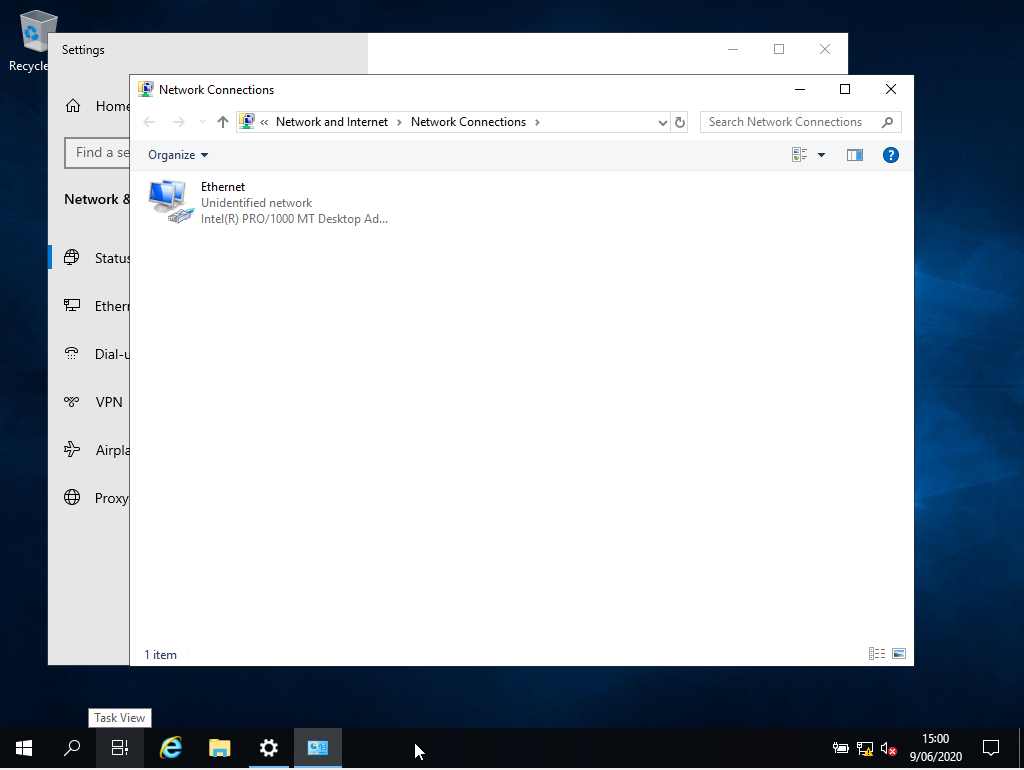
\includegraphics[height=0.40\textheight]{Port_no_network_access.png}
	\caption{Deze afbeelding geeft aan dat het apparaat niet met het netwerk is verbonden, wanneer men aansluit op één van de poorten op de Cisco switch.}
\end{figure}

\begin{figure}[H]
	\centering
	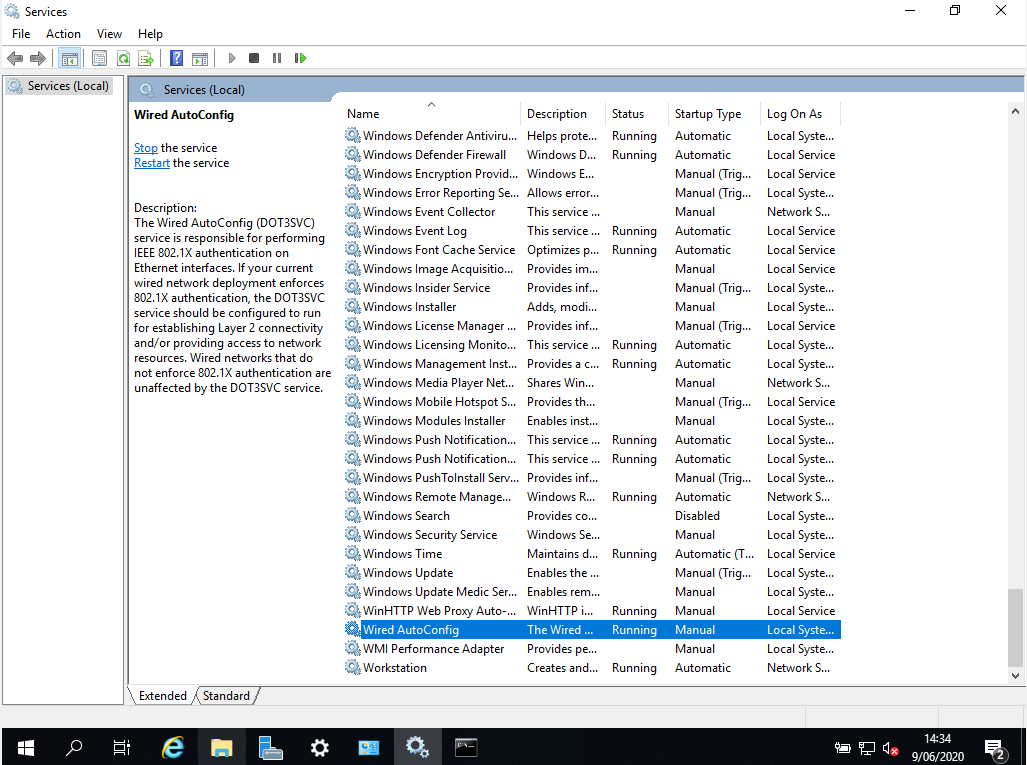
\includegraphics[height=0.40\textheight]{Service_ise_port.png}
	\caption{Deze afbeelding geeft de service 'Wired AutoConfig' weer.}
\end{figure}
\newpage
Het is echter wanneer men de 'Wired AutoConfig' services aanzet, kan men zich aanmelden op het netwerk door volgende stappen uit te voeren: 
\newline

\begin{itemize}
	\item Open het configuratiescherm, en ga naar 'netwerk en internet'.
	\item Open vervolgens het 'netwerkcentrum'.
	\item Open 'Adapter instellingen wijzigen'.
	\item Open het 'properties' tablad, door rechtermuisklik op de  correcte "Ehternet adapter".
	\item Vervolgens ziet men het tablad "Authenticatie".
	\item Open "Extra instellingen".
	\item Veranderd het de 'authentication modus' naar gebruikers authenticatie.
	\newline
\end{itemize}


Het is echter wanneer men het juiste gebruikersnaam en wachtwoord ingeeft, dan wordt de gebruiker met zijn apparaat aangesloten op het netwerk. Vervolgens is ook een policy rule geïmplementeerd dat alleen gebruikers van de groep 'Employees' kunnen aanmelden op het netwerk via één van de Cisco poorten. Dit werd echter al eerder vernoemd in het proof of concept hoofdstuk. 
\newline
\newline
Het is enigszins duidelijk dat wanneer men wenst in te loggen met de gebruiker 'Test' en het wachtwoord 'Admin2020', dat men geen toegang krijgt tot het netwerk. Dit komt omdat gebruiker 'Test' zich niet in de groep 'Employees' bevindt. Hierdoor is aangetoond dat het gebruik van policies ook de vruchten plukt op beveiliging.

\begin{figure}[H]
	\centering
	\subfloat{{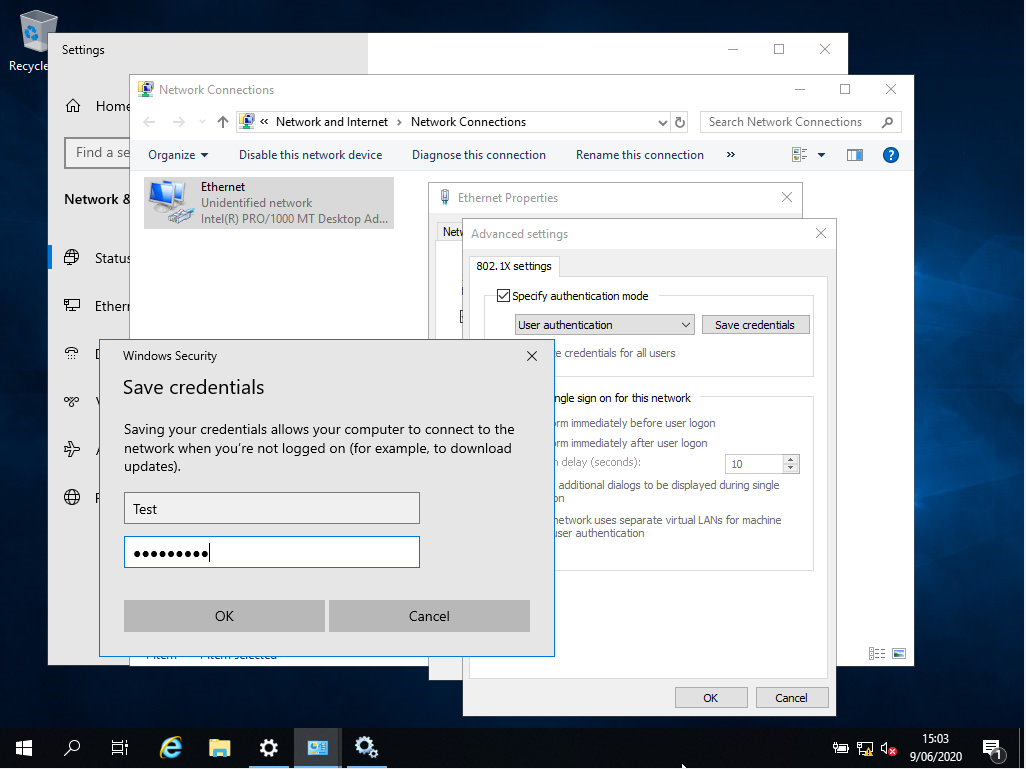
\includegraphics[width=6.5cm]{Test_no_employee.png} }}%
	\qquad
	\subfloat{{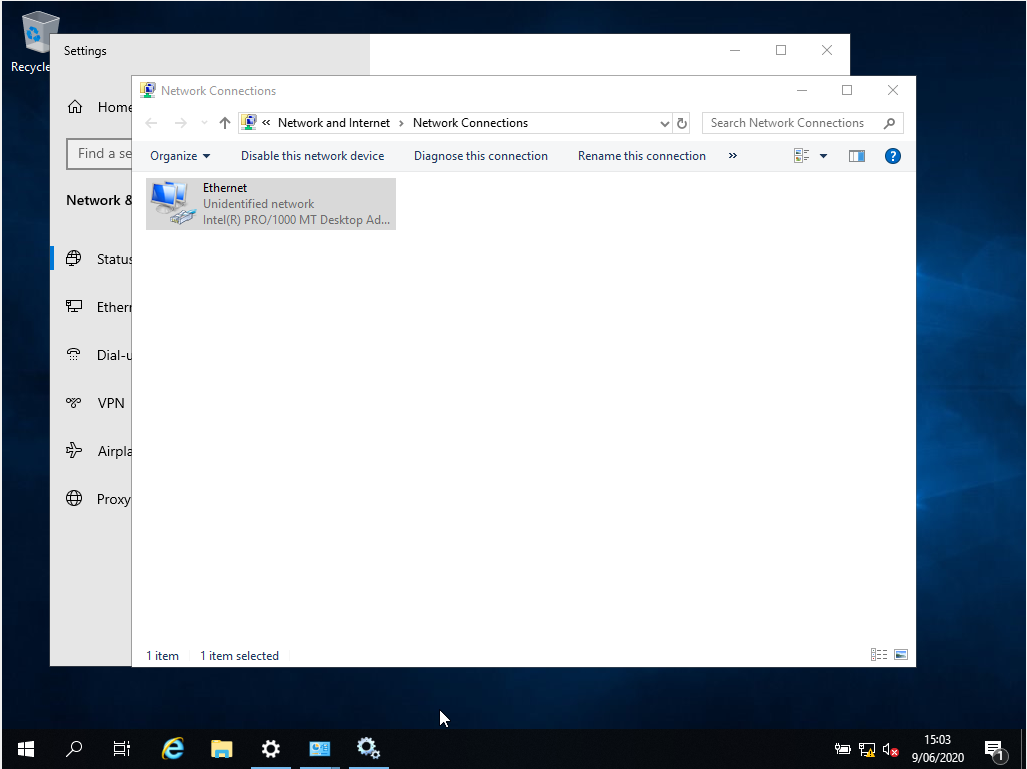
\includegraphics[width=6.5cm]{Test_no_successed.png} }}%
	\newline
	\qquad
	\subfloat{{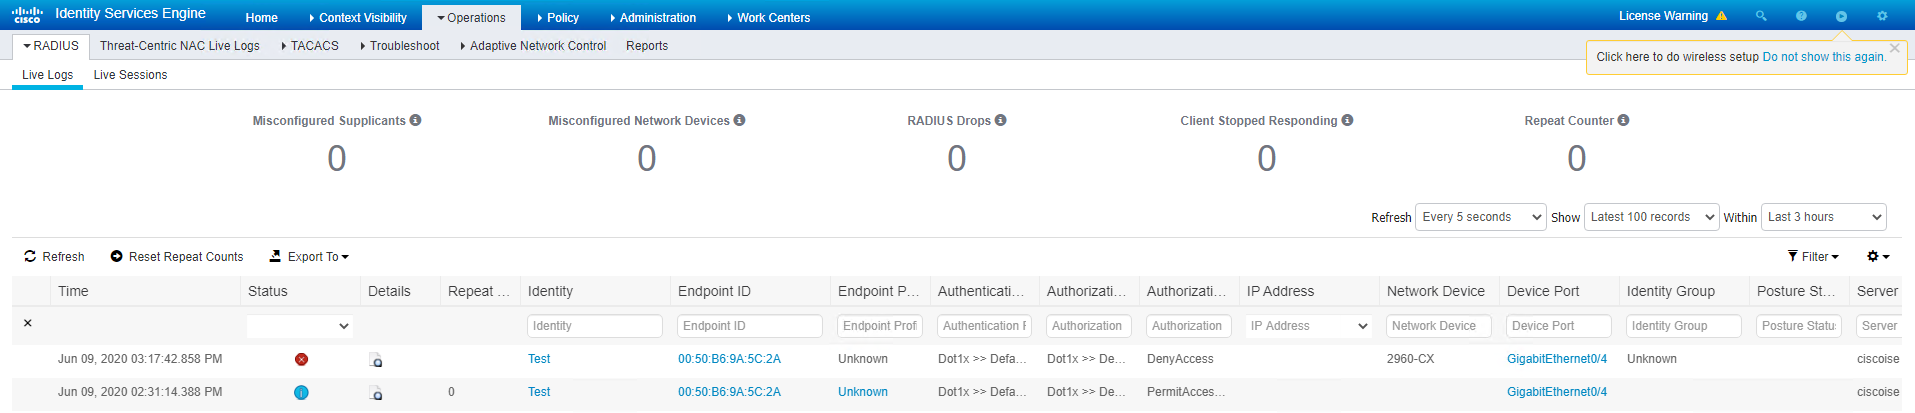
\includegraphics[width=14cm]{TestDenied.png} }}%
	\caption{Bovenstaande foto's geven aan dat gebruiker 'Test' zich niet kan aansluiten op het netwerk. Omdat de gebruiker 'Test' niet in de groep 'Employees' bevindt.}%
	\label{fig:Test_gebruiker}%
\end{figure}
	
Als men wenst in te loggen met een gebruiker die zich in de ISE groep 'Employees' bevindt, dan zal deze gebruiker met zijn apparaat via een poort kunnen aansluiten op het netwerk. 
\newline
\newline
Wanneer de test met gebruiker 'TestV2', die zich in de groep 'Employees' bevindt, uitgevoerd wordt. Dan is het vanzelfsprekend dat deze gebruiker met zijn apparaat met het netwerk kan verbinden.

\begin{figure}[H]
	\centering
	\subfloat{{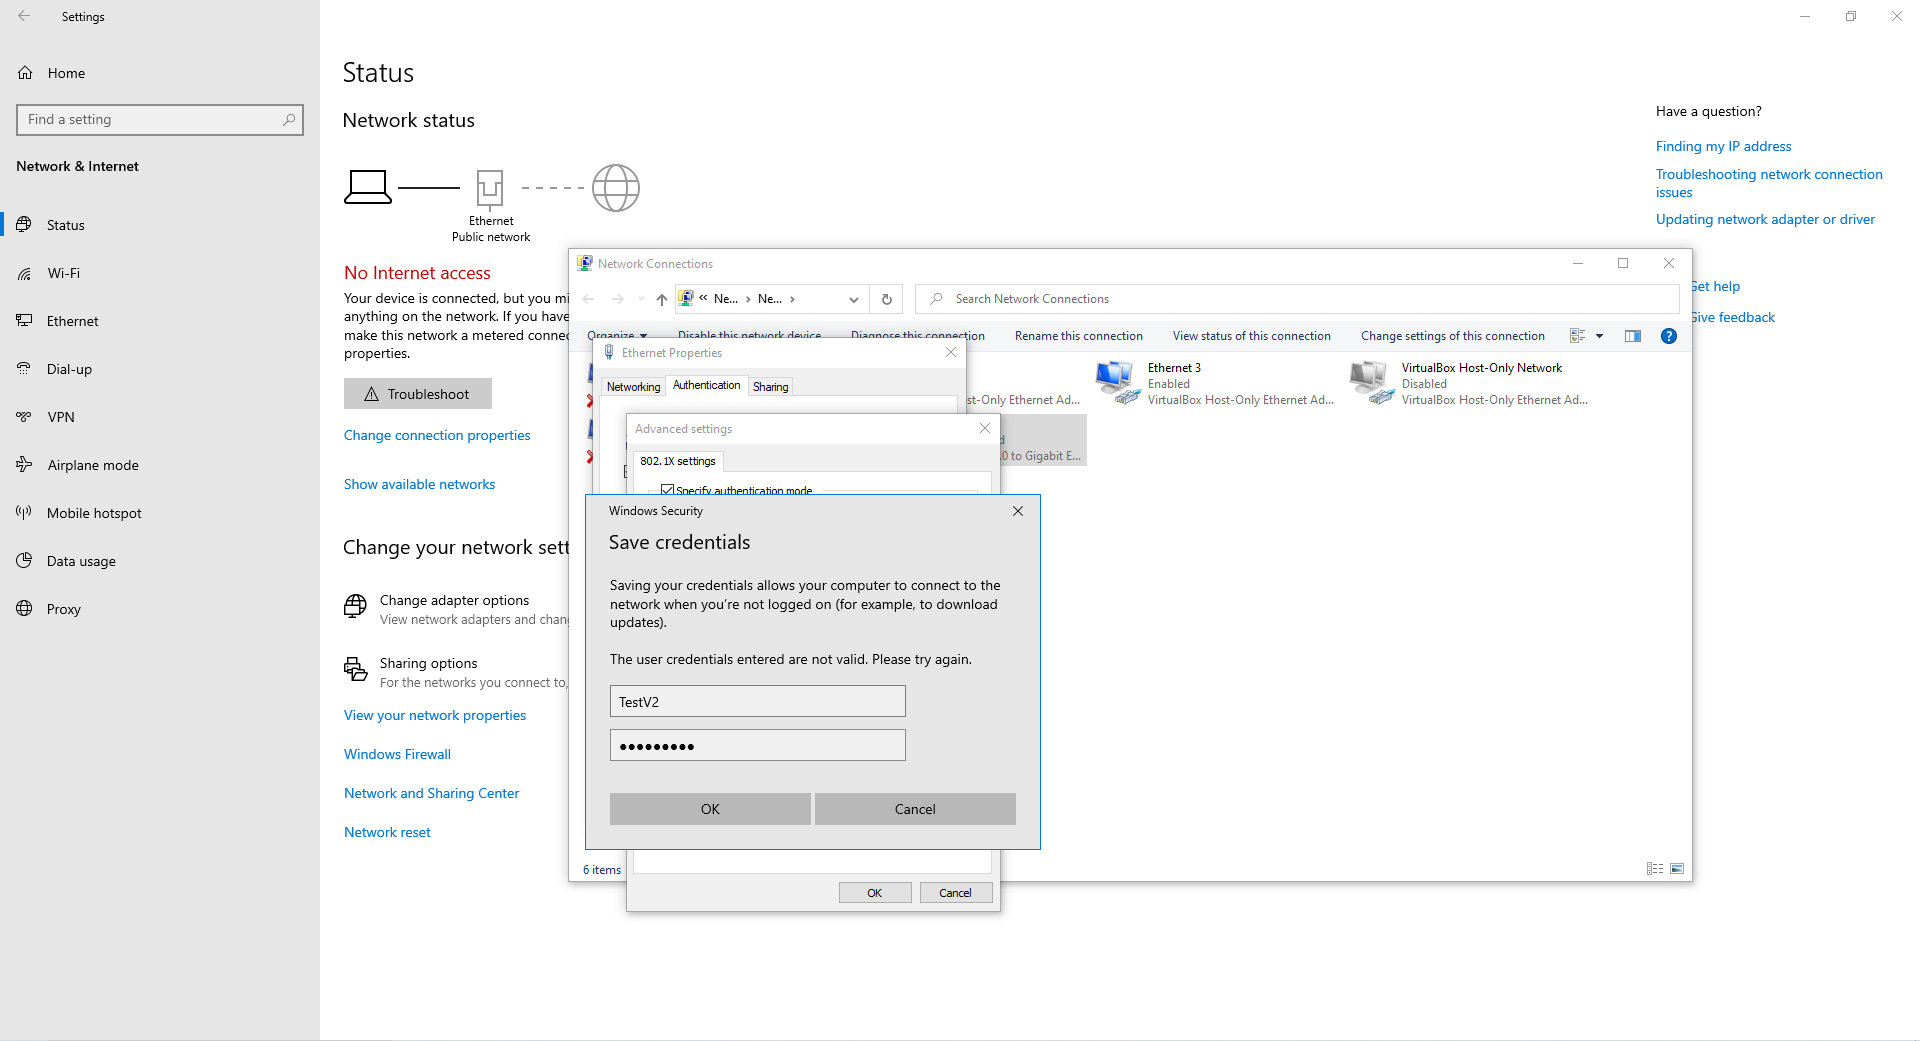
\includegraphics[width=6.5cm]{TestV2_Employee.png} }}%
	\qquad
	\subfloat{{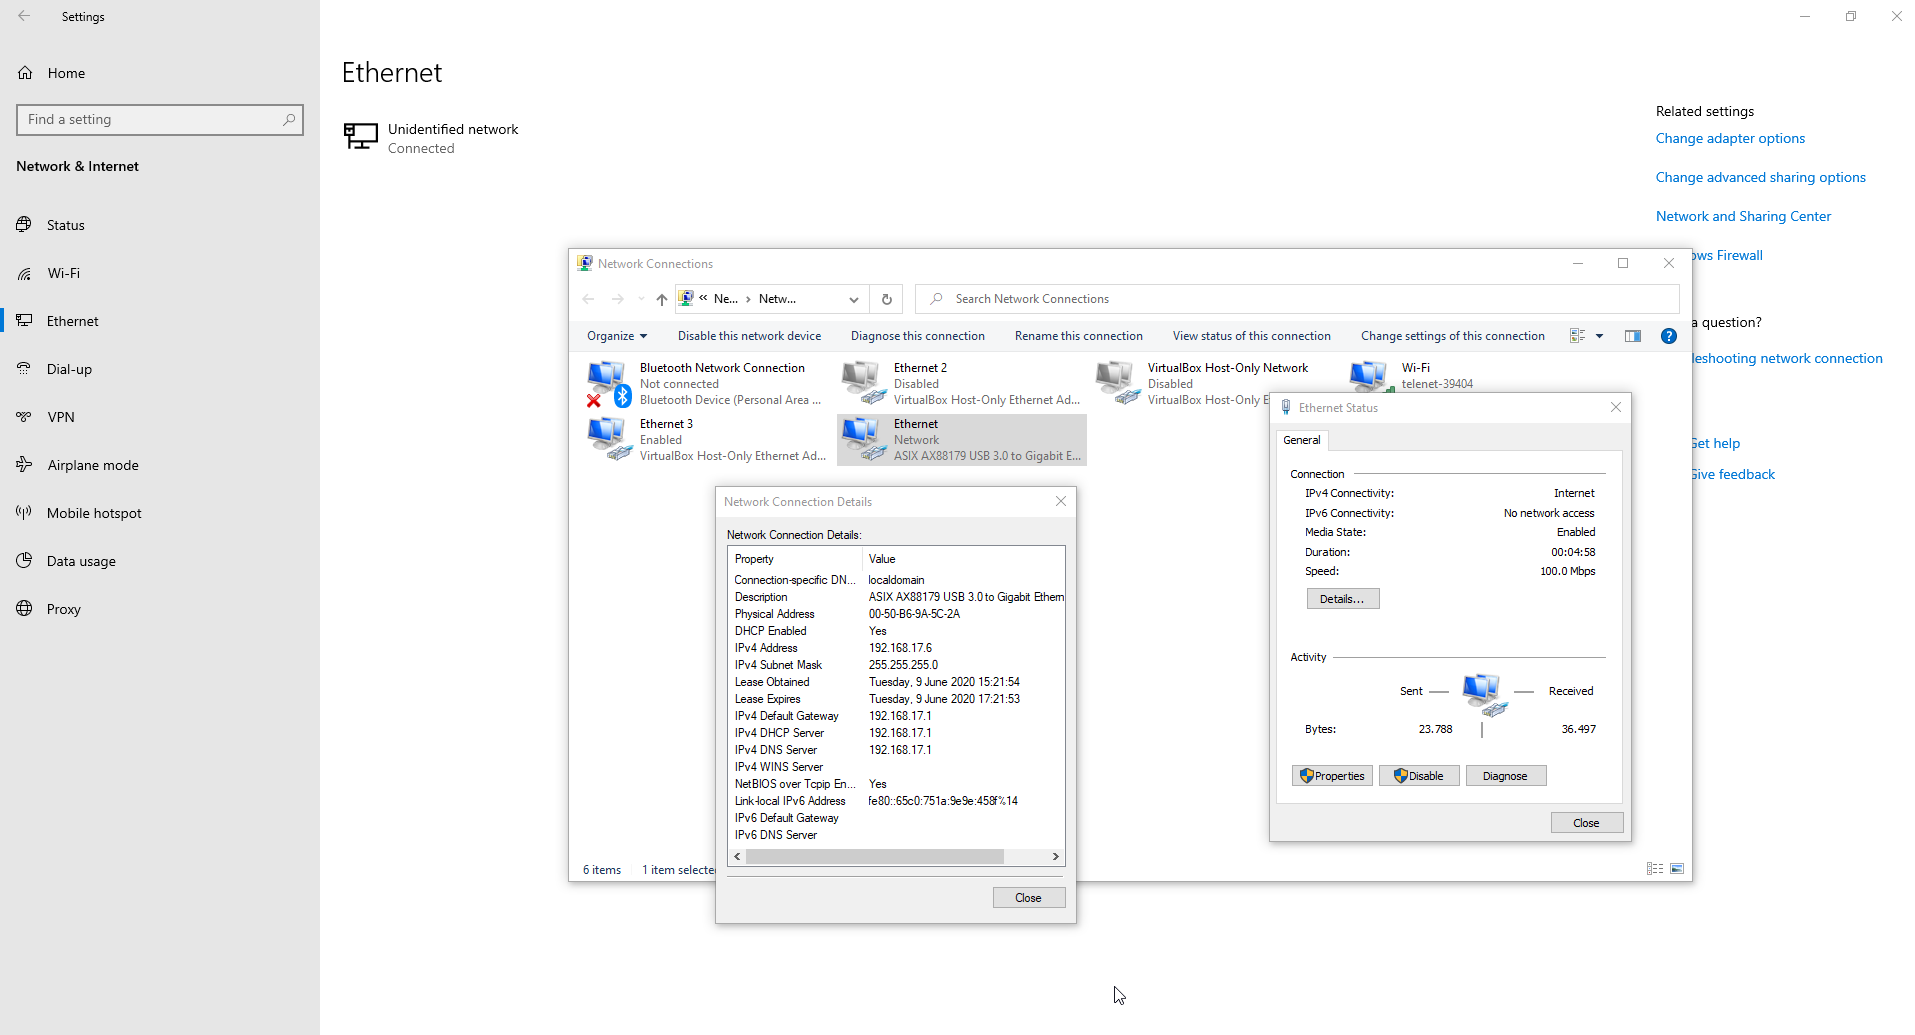
\includegraphics[width=6.5cm]{TestV2_succeeded.png} }}%
	\newline
	\qquad
	\subfloat{{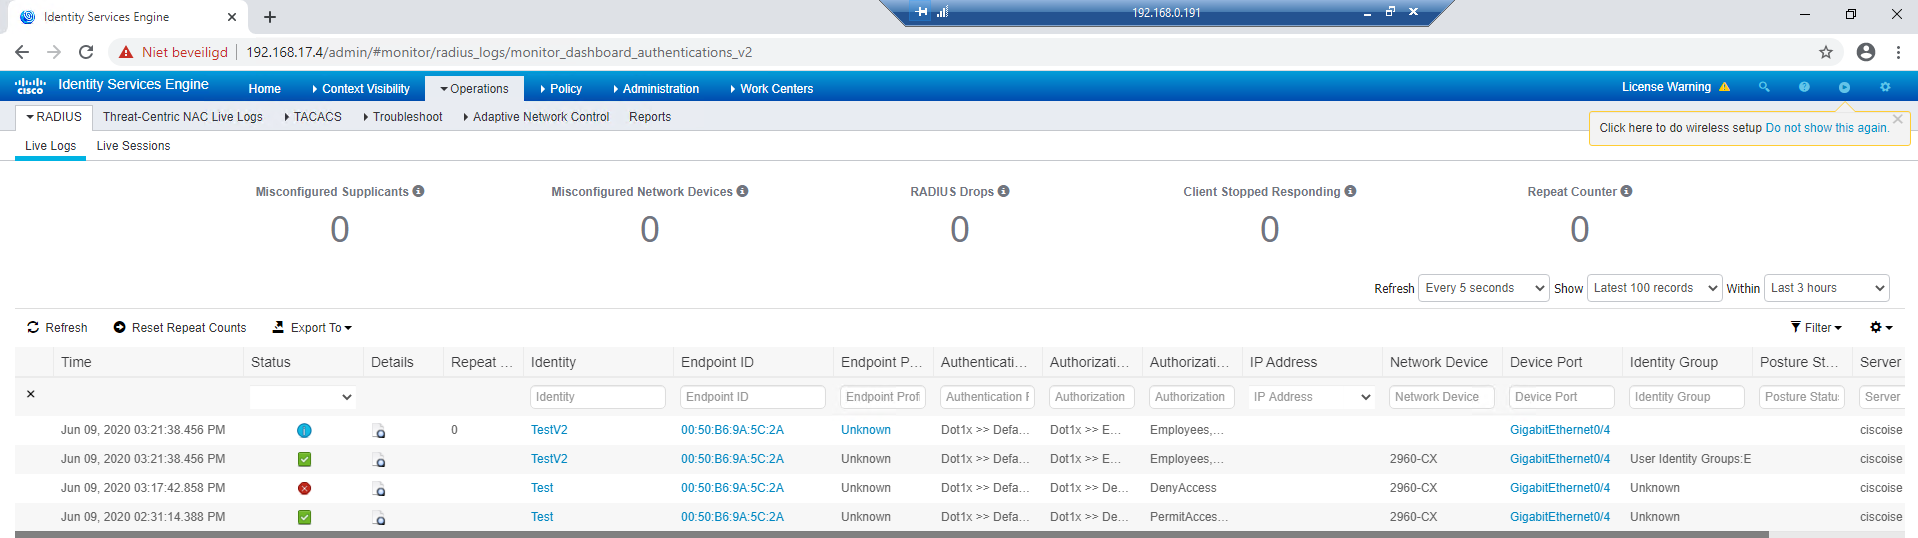
\includegraphics[width=14cm]{TestV2_succeeded_ISE.png} }}%
	\caption{Bovenstaande foto's geven aan dat gebruiker 'TestV2' zich kan aansluiten op het netwerk. Omdat de gebruiker 'TestV2' zich in de groep 'Employees' bevindt.}%
	\label{fig:Test_gebruiker}%
\end{figure}

Hierdoor is aangetoond dat Cisco Idendity Services Engine met use cases 'Port-based en Policy-based network access control' een positieve uitkomst bekomt. M.a.w. plukt 'Port-based en Policy-based network access control' de vruchten af op security vlak. In de volgende subsectie zullen de resultaten van Tread-Centric en Policy-based network access control besproken worden.


\subsection{Tread-Centric en Policy-based network access control}
\section{Cisco Identity Services Engine enquête}

\begin{figure}[H]
	\centering
	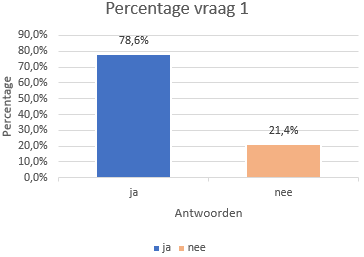
\includegraphics[height=0.30\textheight]{Vraag1.png}
	\caption{Deze afbeelding geeft de service 'Wired AutoConfig' weer.}
\end{figure}

\begin{figure}[H]
	\centering
	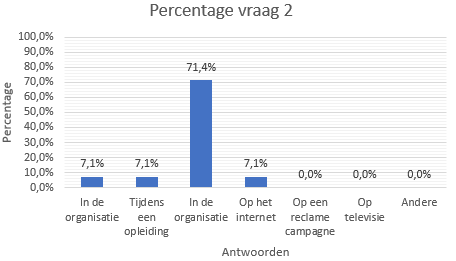
\includegraphics[height=0.30\textheight]{Vraag2.png}
	\caption{Deze afbeelding geeft de service 'Wired AutoConfig' weer.}
\end{figure}

\begin{figure}[H]
	\centering
	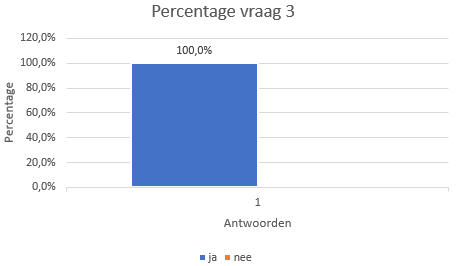
\includegraphics[height=0.40\textheight]{Vraag3.png}
	\caption{Deze afbeelding geeft de service 'Wired AutoConfig' weer.}
\end{figure}

\begin{figure}[H]
	\centering
	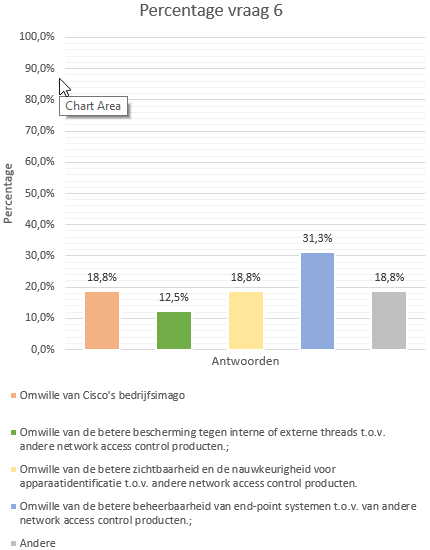
\includegraphics[height=0.30\textheight]{Vraag6.png}
	\caption{Deze afbeelding geeft de service 'Wired AutoConfig' weer.}
\end{figure}

\begin{figure}[H]
	\centering
	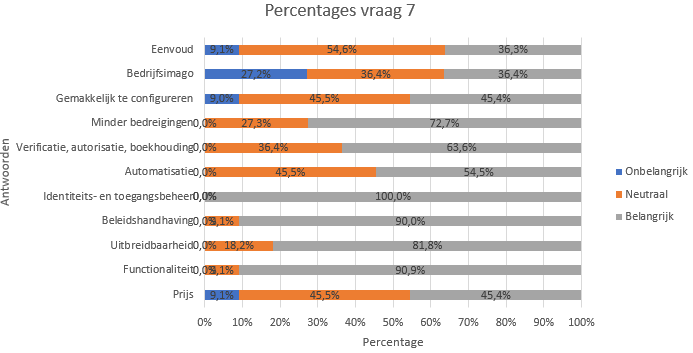
\includegraphics[height=0.30\textheight]{Vraag7.png}
	\caption{Deze afbeelding geeft de service 'Wired AutoConfig' weer.}
\end{figure}

\begin{figure}[H]
	\centering
	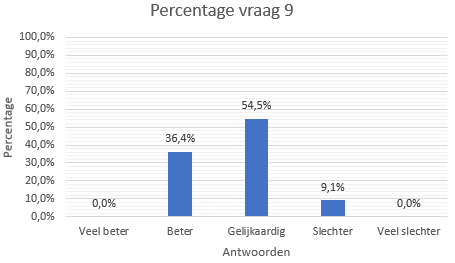
\includegraphics[height=0.30\textheight]{Vraag9.png}
	\caption{Deze afbeelding geeft de service 'Wired AutoConfig' weer.}
\end{figure}

\begin{figure}[H]
	\centering
	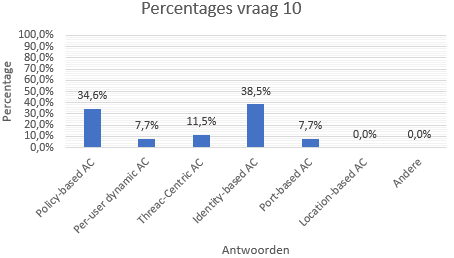
\includegraphics[height=0.30\textheight]{Vraag10.png}
	\caption{Deze afbeelding geeft de service 'Wired AutoConfig' weer.}
\end{figure}

\begin{figure}[H]
	\centering
	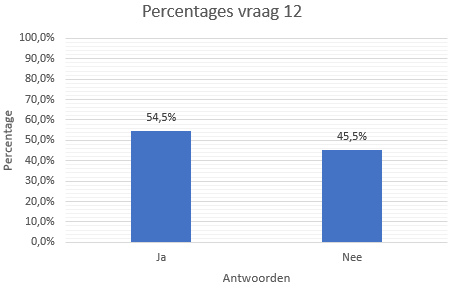
\includegraphics[height=0.30\textheight]{Vraag12.png}
	\caption{Deze afbeelding geeft de service 'Wired AutoConfig' weer.}
\end{figure}
\begin{figure}[H]
	\centering
	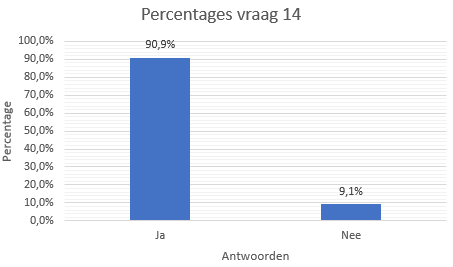
\includegraphics[height=0.30\textheight]{Vraag14.png}
	\caption{Deze afbeelding geeft de service 'Wired AutoConfig' weer.}
\end{figure}
\begin{figure}[H]
	\centering
	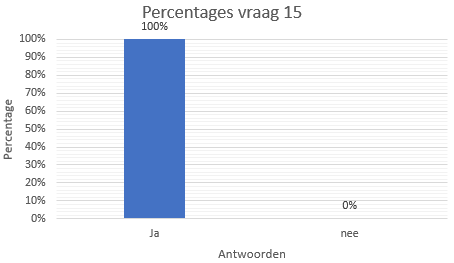
\includegraphics[height=0.30\textheight]{Vraag15.png}
	\caption{Deze afbeelding geeft de service 'Wired AutoConfig' weer.}
\end{figure}
\begin{figure}[H]
	\centering
	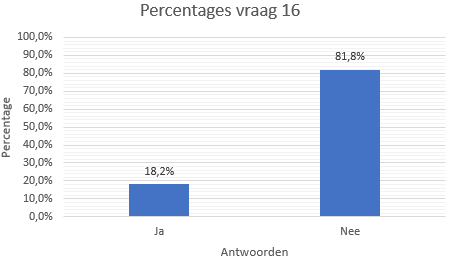
\includegraphics[height=0.30\textheight]{Vraag16.png}
	\caption{Deze afbeelding geeft de service 'Wired AutoConfig' weer.}
\end{figure}
\begin{figure}[H]
	\centering
	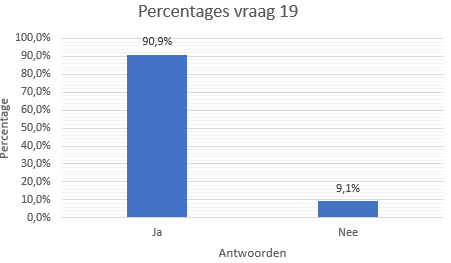
\includegraphics[height=0.30\textheight]{Vraag19.png}
	\caption{Deze afbeelding geeft de service 'Wired AutoConfig' weer.}
\end{figure}
\begin{figure}[H]
	\centering
	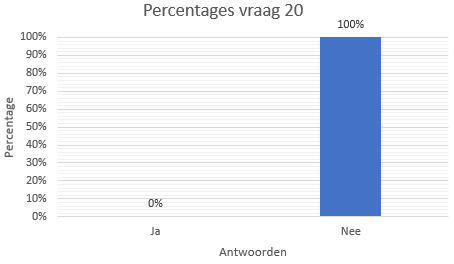
\includegraphics[height=0.30\textheight]{Vraag20.png}
	\caption{Deze afbeelding geeft de service 'Wired AutoConfig' weer.}
\end{figure}

